\section{Usage}
\label{sec:usage}

This section is intended to demonstrate some of the basic \LaTeX\ commands and features you may
find helpful to be familiar with. This is likely not a comprehensive list, so please do go looking
for other features and packages that you think you may find helpful. As with everything else,
Stack Overflow is the best teacher there is!

\subsection{Using Images}

Throughout your project writeup, you will need to include figures, such as
Figure~\ref{fig:stack_overflow} below. This is generally done using the \verb|\includegraphics{}|
command. However this doesn't include \verb|.svg| files, so the \verb|\includesvg{}| command from
the \verb|svg| library should be used in that case instead. Wherever possible, you should aim to
use vector graphic formats such as \verb|svg| or \verb|pdf| to ensure there's no chance of low
resolution, hard to read images in your writeup.

\begin{figure}[ht]
	\centering
	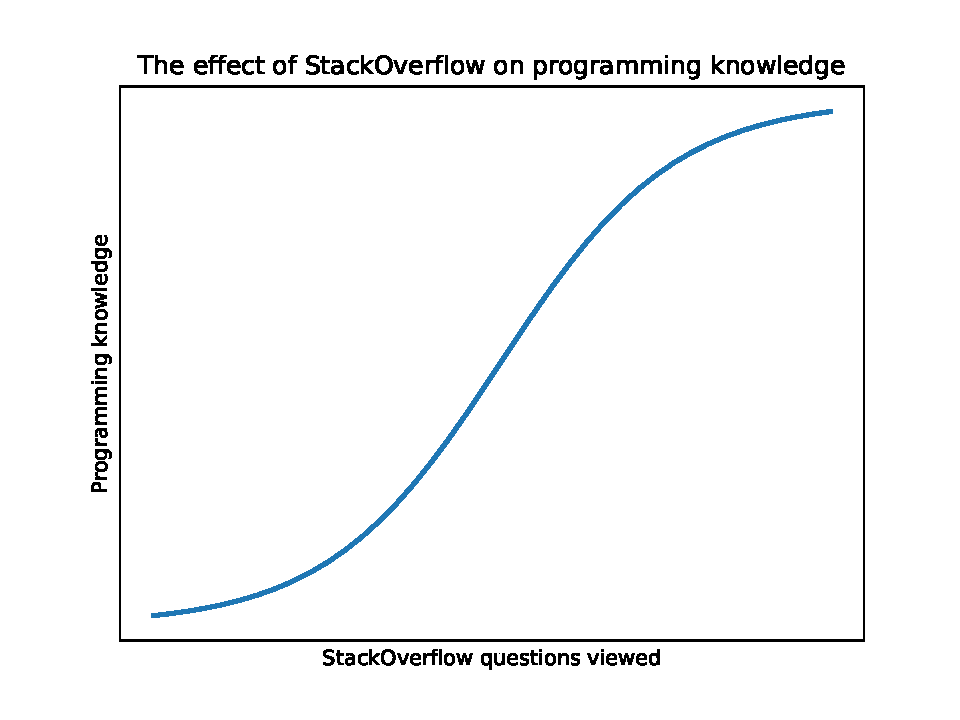
\includegraphics[width = 0.8\textwidth]{figures/stackoverflow_plot.pdf}
	\caption{A plot of \acrlong{cs} knowledge against Stack Overflow use}
	\label{fig:stack_overflow}
\end{figure}

\subsection{Using Tables}

You can see below a short list of some of the more helpful \LaTeX\ commands to know, as well as a
demonstration of how to use tables. It's okay if not all of these are helpful to you, but it may
be a good starting point for things to be aware of.

\todo[inline]{Fix latexindent on this table}
\begin{table}[ht]
	\centering
	\begin{tabular}{|p{0.15\linewidth}|p{0.70\linewidth}|}
		\hline
		\verb|\cite|  & Insert a citation using the bibliography key in your \verb|references.bib| file                              \\
		\hline
		\verb|\label| & Add a point that can be referenced elsewhere in the document, such as on a section heading, figure, or table \\
		\hline
		\verb|\ref|   & Add a reference to a label elsewhere in the document. You should precede
		this with \verb|~|, which is a whitespace that won't be split across new lines.                                              \\
		\hline
		\verb|\SI|    & Add a number formatted with SI units e.g., \verb|\SI{5}{\kilo\byte}| = \SI{5}{\kilo\byte}                    \\
		\hline
		\verb|\verb|  & An inline way to render text exactly as written in a monospace font, like the commands in this table.        \\
		\hline
	\end{tabular}
\end{table}

\subsection{Other features}

Throughout this template, I've also used a few other features that you ought to make use of, but
which weren't big enough to deserve a whole subsection. You're encouraged to go out looking for
them throughout this template to get a handle on how to use them. Some are also mentioned in the
table above with explanations of how they can be used.

\begin{itemize}
	\item Citations
	\item Acronyms
	\item References to sections and figures
	\item Lists and enumerations
\end{itemize}
